\documentclass{vldb}
\usepackage{graphicx, subfigure}
\usepackage{balance, url, amsfonts, verbatim, mathtools}  % for  \balance command ON LAST PAGE  (only there!)

\title{Probabilistically Bounded Staleness and\\ Practical Partial Quorum Systems}

\newdef{definition}{Definition}

\begin{document}

\interfootnotelinepenalty=10000
\hyphenation{prob-a-bil-is-tic-ally}

\maketitle

\noindent\textit{``All good ideas arrive by chance.''--Max Ernst}


\begin{abstract}

Modern storage systems employing quorum replication are often
configured to use partial, non-strict quorums.  These systems wait
only for a subset of their replicas to respond to a request before
returning an answer, without guaranteeing that read and write replica
sets intersect.  While these partial quorum mechanisms provide only
basic eventual consistency guarantees, with no limit to the recency of
data returned, these configurations are frequently ``good enough'' for
practitioners given their latency benefits. In this work, we discuss
why partial quorums are often acceptable in practice by analyzing the
staleness of data they return.  Extending prior work on strongly
consistent probabilistic quorums and using models of Dynamo-style
anti-entropy processes, we introduce Probabilistically Bounded
Staleness (PBS) consistency, which provides expectations of bounds on
staleness across both versions and wall clock time.  We derive a
closed-form solution for versioned staleness and model real-time
staleness for representative Dynamo-style systems under internet-scale
production workloads.  We quantitatively demonstrate why, in practice,
systems employing partial quorums often serve consistent data.

\end{abstract}


\section{Introduction}

Modern distributed storage systems need to be scalable, highly
available, and provide high performance for reads and writes.  These
systems typically replicate data across different machines or even
across datacenters for two reasons: first, to provide high
availability when components fail and second, to provide improved
performance by serving requests from multiple replicas.  In order to
provide predictably low read and write latency, systems often eschew
consistency across replicas and instead provide eventual
consistency. In this model, replicas are only guaranteed to eventually
agree on the value of a particular data item, and reads may return
arbitrarily stale data.

Distributed quorums are often used to ensure strong consistency across
multiple replicas of a data item by overlapping read and write
sets. However, service latency is critical. For example, at Amazon,
100 ms of additional latency resulted in 1\% drop in
sales~\cite{amazon-latency}, while 500 ms of additional latency at
Google due to increasing the number of search results computed
resulted in a corresponding 20\% decrease in search
traffic~\cite{google-talk}.  At scale, these decreases correspond to
billions of dollars of lost revenue.

One technique for lowering operation latency is employing
\textit{partial or partial quorums}, in which read and write sets
are not guaranteed to overlap (given $N$ replicas and read and write
quorum sizes $R$ and $W$, $R+W \leq N$).  Modern quorum-based scalable
data systems such as Dynamo~\cite{dynamo} (and its open source
descendants Cassandra~\cite{cassandra}, Riak~\cite{riak}, and
Voldemort~\cite{voldemort}) provide two categories of quorum
operation: overlapping quorums and strong consistency or
variable-sized partial quorums with no guarantees on the staleness or
consistency returned, other than that the system will ``eventually''
provide the most recent version in the absence of new writes.  Despite
these weak guarantees, operators frequently employ partial
quorums--they are often ``good enough'' for applications, especially
given their latency benefits.

Prior work evalued the probability of strong consistency for static
partial quorum systems, where, in the absence of failures, the read
and write sets do not change over time.  Theoretical research on
\textit{probabilistic quorums} demonstrated how partial quorums can be
employed to provide arbitrarily high probability of strong
consistency~\cite{prob-quorum}. In theory, these systems provide
excellent asymptotic behavior but are limited in practical
applicability due to their reliance on high replication factors.  More
problematic, however, is that this work predicts \textit{how often} a
response will be stale but not \textit{how stale} a stale response
will be. In the real world, quorum systems are not static: writes
propagate asynchronously across time. Similarly, as evidenced by the
widespread deployment of eventually consistent data systems,
applications can tolerate varying degrees of staleness.

In this paper, we present algorithms and models for accurately
predicting the staleness of partial quorums across multiple versions
and wall clock time, or Probabilistically Bounded Staleness (PBS). PBS
can be used to determine the probability of reading one of the last
$k$ versions of a data item ($k$-staleness), of reading a data item
$t$ seconds after it is written ($t$-visibility), and of experiencing
a combination of the two ($\langle k, t \rangle$-staleness).  We also use these
consistency measures to provide probabilistic guarantees on monotonic
reads, a form of session guarantees where reads are guaranteed to
return data items no older than what has been previously read.

Observing multi-version staleness is highly unlikely.  Under static
quorum systems, the probability of returning a version $k$ versions
older than the most current is exponentially reduced by a factor of
$k$.  In the presence of multiple concurrent writes in a non-static
system, there is a similar effect, determined in large part by the
staggering of the writes.  With a modest global write rate to a key, a
client making read requests no greater than the write rate has a high
probability of observing monotonic reads consistency.  Many
applications can tolerate stale versions, particularly programs
exposing append-only data structures such as logs and streaming
timelines and, more generally, commutative updates.

Observing staleness across time depends on the write propagation rate
and the latency between coordinators and replicas.  In this paper, we
examine Dynamo-style partial quorums, which are currently the most
widely deployed quorum replication strategy.  We show how staleness in
the Dynamo model is dependent on message reordering and discuss the
effect of latency variance on expected staleness across time.
Additionally, we propose asynchronous staleness detectors within
Dynamo.  We present algorithms for both a simple detector that is
easily implementable within Dynamo but may provide false positives and
a more complex, precise detector.  Using data collected in experiments
on Amazon's EC2 and using production distributions provided by two
internet-scale companies, we analyze the likelihood of $t$-staleness
across time and replica configurations.



We make the following contributions in this paper:

\begin{itemize}

\item We develop the theory of Probabilistically Bounded Staleness
  (PBS) for partial quorums. PBS describes staleness probability
  metrics across both versions ($k$-staleness) and time
  ($t$-visibility) as well as probabilistic monotonic reads
  consistency.

\item We provide a closed-form analysis of $k$-staleness demonstrating
  how the probability of receiving data $k$ versions stale is
  exponential in $k$ for static quorums.  $k$-staleness tolerance also
  exponentially lowers formally-defined quorum system load.

\item We provide a model for $t$-visibility in
  Dynamo-style partial quorum systems, showing how
  staleness is dependent on message reordering in the system.  We
  evalute the $t$-visibility of Dynamo-style systems using a
  combination of experimentally-gathered data and production traces.

\end{itemize}

The remainder of this paper is as follows: in
Section~\ref{sec:background}, we provide an overview of quorum systems
and Dynamo-style quorums.  In Section~\ref{sec:pbs}, we introduce
Probabilistically Bounded Staleness and provide a closed-form solution
to $k$-staleness under traditional static quorums.  In
Section~\ref{sec:dynamo}, we model Dynamo-style quorum systems and
discuss when staleness occurs.  In Section~\ref{sec:dynamoeval}, we
use real-world workloads and Monte Carlo analysis to determine how often Dynamo-style quorums return stale values in practice.  In Section~\ref{sec:discussion}, we describe further improvements to dynamic partial quorums, in Section~\ref{sec:relatedwork}, we discuss related work, and, in Section~\ref{sec:conclusion}, we conclude.


\section{Background}
\label{sec:background}

\subsection{Quorum Foundations: Theory}

Quorum systems have long been proposed as a replication strategy for
distributed data storage.  Informally, a strict quorum system defines
a set of sets of nodes in a distributed system with the property that
any two sets in the quorum system overlap (have non-empty
intersection).  When considering distributed get/put operations,
reading and writing to sets of nodes in a strict quorum system ensures
strong consistency in the absence of failures; the minimum sized
quorum defines its fault tolerance.  A simple example of a strict
quorum system is the majority quorum system, in which each quorum is
of size $\frac{N}{2}+1$.  However, the theory literature contains
numerous alternative quorum systems providing varying asymptotic
properties of capacity, scalability, and fault-tolerance, from
tree-quorums to grid-quorums.  Jim\'{e}nex-Peris et. al provide a
useful overview of these traditional, strict quorum
systems~\cite{quorums-alternative}.

Partial quorum systems are a natural extension of strict quorum
systems: at least two sets in a partial quorum system do not
overlap.  There are two relevant variants of partial quorum systems in
the literature: probabilistic quorum systems and k-quorums.

\textit{Probabilistic quorum systems} provide probabilistic guarantees
on the consistency of data returned by partial quorums.
Probabilistic quorums provide optimal (expected) load and fault
tolerance with an arbitrarily small probability of
inconsistency~\cite{prob-quorum}.  Intuitively, this is a consequence
of the Birthday Paradox: as the number of replicas increases, the
probability of non-overlap between any two subsets is quite low.  To
the best of our knowledge, probabilistic quorums have only been used
to study the probability of strong consistency and have not been
employed in an eventually consistent context.

Given $n$ replicas and randomly chosen read and write quorums of sizes
$r$ and $w$, we can calculate the probability of the read quorum not
containing the value written by the write quorum.  The probability of
staleness is the number of quorums of size $r$ composed of nodes that
were not written to in the write quorum divided by the number of
possible quorums of size $r$:
\begin{equation}
\label{eq:prob-strict}
p_{stale}=\frac{{n-w \choose r}}{{n \choose r}}
\end{equation}
It is readily apparent that the probability of staleness is quite high
except for large values of $n$.  With $n=100$, $r=w=30$, $p_{stale} =
1.88 \times 10^{-6}$~\cite{nonstrict-availability}.  However, with
$n=3$, $r=w=1$, $p_{stale} = .\overline{6}$.  The asymptotics of these
systems are excellent---but only asymptotically.  

\textit{$k$-quorum systems} provide strong \textit{deterministic}
guarantees that the partial quorum system will return a value that was
written within $k$ versions of the most recent
write~\cite{nonstrict-availability}.  In the single-writer scenario,
one can imagine a round-robin write scheduling scheme where each write
is sent to $\frac{n}{K}$ replicas such that each replica is no more
than $K$ versions out-of-date.  However, with multiple writers, one
loses the ordering properties that the single-writer was able to
control, and the best known algorithm for the pathological case
results in a lower bound of $(2n-1)(k-1)+n$ versions staleness~\cite{k-quorum-lb}.

This prior work has two properties with important implications for
practitioners.  First, existing theory treats quorums as static; a
write quorum is chosen and no other replicas in the system
subsequently learn about the value unless it is written again.  The
theory does not account for propagation of versions across time and
between replicas (anti-entropic processes).  Second, much of this
prior work assumes Byzantine failure.  If the description of prior
work seemed simplistic, it is largely because most of the literature
content addresses problems such as adversarial quorum selection and
scheduling.  In this work, we re-evaluate both of these assumptions.  We
elaborate further in the next subsection.

\subsection{Quorum Foundations: Practice}
\label{sec:practice}

In practice, many distributed data management systems use quorums as a
replication strategy. Amazon's Dynamo~\cite{dynamo} is the progenitor
of a class of eventually-consistent key-value stores using a
particular variant of quorum-style replication that includes Apache
Cassandra, Basho's Riak, and LinkedIn's Voldemort\footnote{Other
  BASE-style systems may employ master-slave replication, as in Apache
  HBase~\cite{hbase}.}.  In this paper, we discuss Dynamo-style quorum
systems largely because we are not aware of any significally
different, widely adopted data systems using quorum replication.
However, with some work, we believe that other systems can adopt our
methodology.  Similarly, we focus on key-value stores as the
aforementioned systems provide some variant of key-value architecture
and do not provide full relational semantics.  Quorum systems may be
employed in RDBMS replication, but, for simplicity, we describe
key-value stores here.

Dynamo-style quorum systems employ one quorum system per key,
typically maintaining the mapping of values to a set of nodes using a
consistent-hashing scheme or a centralized membership protocol. Each
node acts as a replica for multiple keys.  Client read and write
requests are sent to a node in the system cluster, which may be
subsequently forwarded to all nodes assigned to that key as replicas.
The coordinating node considers an operation complete when it has
heard from a pre-defined number of replicas.  In Dynamo terminology,
the quorum size, or replication factor, is defined as $N$, the number
of replica responses required for a successful read is defined as $R$,
and the number of replica acknowledgements required for a successful
write is defined as $W$. Dynamo-style systems return guaranteed
strongly consistent data when $R+W > N$.  Setting $W>\lceil N/2 \rceil$ accounts for
the possibility of concurrent outstanding write requests overlapping.

For improved latency, operators often set $R+W \leq N$.  Cassandra's
default configuration is $N$$=$$3$, $R$$=$$W$$=$$1$.  Riak defaults
to $N$$=$$3$,$R$$=$$W$$=$$2$.  Voldemort does not provide sample
configurations, but Voldemort's authors at LinkedIn often choose $N$$=$$c$,
$R$$=$$W$$=$$ \lceil c/2 \rceil$ for odd $c$.  However, for applications
requiring ``very low latency and high availability'', LinkedIn uses
Voldemort with $N$$=$$3$, $R$$=$$W$$=$$1$.  For other applications, LinkedIn uses
Voldemort with $N$$=$$2$, $R$$=$$W$$=$$1$, providing ``some consistency'',
particularly when $N$$=$$3$ replication si not required.  Note that
Voldemort supports a concept of preferred reads and writes, meaning it
will block until either the preferred number of replicas respond or a
timeout occurs.  In the low latency case, preferred reads is either
two or is disabled.  In the $N$$=$$2$ case, preferred reads and preferred
writes are set to two.

\begin{figure}
\centering
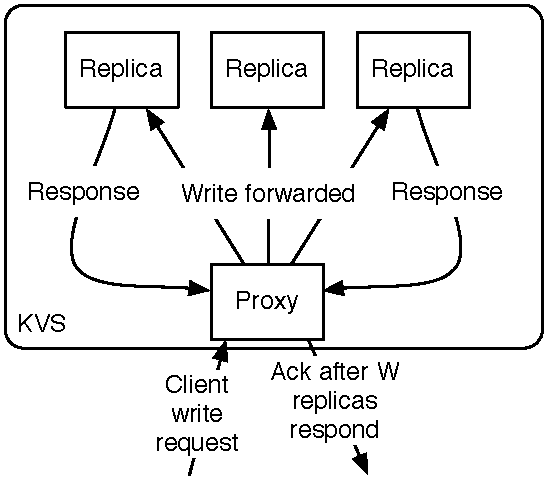
\includegraphics[width=.8\columnwidth]{figs/dynamo-quorum.pdf}
\caption{Diagram of control flow for client write to Dynamo-style
  quorum.  Here, $N=3$, $W=2$. The client write is handled by a
  coordinator node and sent to all replicas. The write succeeds when
  $W$ replicas respond.  Note that the coordinator is possibly a
  replica as well, invoking a local write.}
\label{fig:dynamo-quorum}
\end{figure}

Many Dynamo-style systems also support additional anti-entropic
processes.  One common feature is called ``read repair'''.  When a
read coordinator receives multiple versions of a data item from
different replicas in response to a read request, it will attempt to
(asynchronously) update the out-of-date replicas with the most recent
version.  The effect of read repair on version drift between replicas
is perhaps unsurprisingly dependent on the read rate.  The original
Dynamo paper used Merkle trees to summarize and exchange data contents
between replicas as a means of secondary anti-entropy (after the
initial write to $N$ replicas).  While open source Dynamo-style
systems use Merkle trees, not all actively employ them in gossip-based
anti-entropy.  For example, Cassandra only executes Merkle tree
anti-entropy when it is manually requested (e.g., \texttt{nodetool
  repair}).

\begin{comment}
\url{http://wiki.apache.org/cassandra/Operations#Repairing_missing_or_inconsistent_data}
\end{comment}

There are significant differences between data systems and the theory
describing quorum operation.  First, replication factors for
distributed data systems are relatively low.  Typical replication
factors are between one and three, however the systems literature has
discussed replication up to a factor of 10~\cite{chain-replication}.
Second, (in the absence of failure), in Dynamo-style partial quorums,
the number of replicas that receive a write increases even after the
operation returns.  This is a simple version of anti-entropy.
Morever, read requests are sent to all replicas, however only the
first $R$ responses are considered.  Third, these systems are often
deployed in a trusted or semi-trusted computing environment; there may
be adversarial threats against data integrity and denial-of-service
attacks, but the underlying computing hardware is
non-adversarial. Within a controlled data center, the failure modes
are certainly reduced from the Byzantine case, and, despite its many
risks, the adversarial failures covered by prior theory appear
unlikely in emerging ``cloud computing'' environments~\cite{needed}.


\section{Probabilistically Bounded\\Staleness}
\label{sec:pbs}

In this section, we introduce the theory of Probabilistically Bounded
Staleness to describe the consistency that existing eventually
consistent data stores provide.  PBS extens of prior work on
probabilistic quorums by accounting for staleness of both versions and
across time.  We introduce the notions of PBS $k$-quorums, which
stochastically bounds the staleness of versions returned by read
quorums, PBS $t$-visibility, which stochastically bounds the time
before a committed version appears to readers, and PBS $<k,
t>$-quorums, a combination of the two prior models.


Practical concerns guide the following theoretical contributions.  We
begin by considering a model without anti-entropic processes.
Accordingly, we assume that $w$ ($r$) of $n$ replicas are randomly
selected for each write (read) operation.  We consider a write
``committed'' once it has reached $w$ replicas and the $w$ replicas
respond.  Similarly, we consider fixed $w$, $r$ and $n$ across
multiple operations. Subsequently, we expand our model to consider
write propagation and time-varying $w$ sizes, as is typically the case
in practice.  In this section, we discuss anti-entropy in general,
however we model Dynamo-style quorums in Section
\ref{sec:dynamo-prop}. We discuss further refinements to our
assumptions in Section \ref{sec:discussion}.

\subsection{PBS $k$-quorums}

Probabilistic quorums allow us to determine the probability of
returning the most recent value written to the database, but do not
tell us what happens when the most recent value is not returned.
Here, we determine the probability of returning a value within a
bounded number of versions.  In the following model, we consider
static write quorums (no anti-entropy) and compose multiple
independent write quorums to model the probable overlap of $k$
independent write sets.
\begin{definition}
A quorum system obeys \textit{PBS $k$-quorum consistency} if, with
probability $1-p_{staler}$, at least one value in any read quorum will
have been committed no later than $k$ versions after the latest committed
version when the read begins.
\end{definition}
Versions whose writes that are not yet committed (in-flight) may be
returned by a read in this formulation of probabilistic $k$-quorums
(see Figure \ref{fig:timelines}A).  The $k$-quorum literature defines
these as $k$-regular semantics~\cite{nonstrict-availability}.

\begin{figure}
\centering
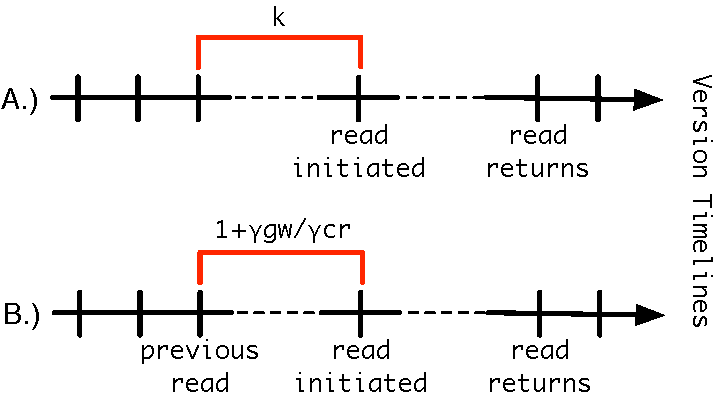
\includegraphics[width=\columnwidth]{figs/timelines.pdf}
\caption{Possible versions returned by read operations under
  PBS $k$-quorums (A) and PBS monotonic reads (B). In
  $k$-consistency, the read operation will return a version no later
  than $k$ versions older than the last committed value when it
  started; more versions may be committed during the read and may be
  returned.  In monotonic reads consistency, the staleness depends on
  the number of versions committed since the time the client last
  completed a read.  This is determined by the proportion of client's
  reads to the number of writes committed to the object.}
\label{fig:timelines}
\end{figure}

The probability of returning a version of a key within the last $k$
versions committed is equivalent to intersecting one of $k$
independent write quorums.  If we assume a random quorum choice, the
probability of non-intersection is simply Equation
\ref{eq:prob-strict} exponentiated by $k$:
\begin{equation}
\label{eq:k-consistency}
p_{staler} = \left(\frac{{n-w \choose r}}{{n \choose r}}\right)^k
\end{equation}

For the $n=3, r=w=1$ case, this means that the probability of
returning a version within $2$ versions is $.\overline{5}$, within $3$
versions $.\overline{703}$, and within $5$ versions $> .868$, and $10$
versions $>.98$.  With $n=3, r=1, w=2$ (alternatively, $r=2, w=1$),
these probabilities increase: $k=1 \rightarrow
.\overline{6}$, $k=2 \rightarrow .\overline{8}, k=5 \rightarrow >
.995$.

In the language of the probabilistic quorum literature, we have
constructed a PBS $k$-quorum from $k$ $\varepsilon$-quorum systems
where $\varepsilon \leq \sqrt[k]{p_{staler}}$. This system has load~\cite{needed}
$\geq \frac{1-\varepsilon^{\frac{1}{2k}}}{\sqrt{n}}$, an exponentially
lower bound than a strict probabilistic quorum.  This follows
immediately from~\cite[Corollary 3.12]{prob-quorum}.

This analytical closed form solution holds for static quorums.  For
dynamic quorums, this solution is an upper bound on the probability of
staleness.

\subsection{PBS Monotonic Reads}

With additional information, we can use PBS $k$-quorums to predict
whether a client will ever read staler data than it has already read.
This property, known as \textit{monotonic reads} consistency is a
well-known session guarantee~\cite{sessionguarantees}.

\begin{definition}
\label{def:prob-mr}
A quorum system obeys \textit{PBS monotonic reads consistency} if,
with probability at least $1-p_{staler}$, at least one value in any
read quorum the same version or a newer version than the client's
previously read value, where versions are defined over the global
commit ordering.
\end{definition}

To guarantee that a client sees monotonically increasing versions, it
can continue to contact the same replica~\cite{vogels-defs}, however
this is insufficient to guarantee strict monotonic reads (where the
client reads strictly newer data).  Definition~\ref{def:prob-mr} can
be adapted to acommodate strict monotonic reads (omitted for brevity).

We observe that monotonic reads is a special case of PBS
$k$-quorums where $k$ is determined by a client's rate of reads from a
data item ($\gamma_{cr}$) and the global, system-wide rate of writes
the same data item ($\gamma_{gw}$).  If we know these rates
exactly, the number of versions between client reads is
$\frac{\gamma_{gw}}{\gamma_{cr}}$, as shown in Figure
\ref{fig:timelines}B.  We can calculate the probability of
probabilistic monotonic reads as follows, effectively using Equation
\ref{eq:k-consistency} where $k=\frac{\gamma_{gw}}{\gamma_{cr}}$:

\begin{equation}
\label{eq:prob-mr}
p_{staler} = \left(\frac{{n-w \choose r}}{{n \choose r}}\right)^{\gamma_{gw}/\gamma_{cr}}
\end{equation}
For strict monotonic reads, where we cannot read the version we've
previously read, we exponentiate where
$k=\frac{\gamma_{gw}}{\gamma_{cr}}-1$.  When constructed from $k$
$\varepsilon$-consistent systems (as we have here), this consistency
model has load $\geq \frac{(1-p_{staler}^{\frac{1}{2C}})}{\sqrt{n}}$,
where $C=\frac{\gamma_{gw}}{\gamma_{cr}}$.

In practice, we may not know these exact rates, but, by measuring
their distribution, we can calculate an expected ratio that we can
integrate into these calculations.  By performing appropriate
admission control, operators can control these rates to achieve
monotonic reads guarantees.

\subsection{PBS $t$-visibility}
\label{sec:tvis}


Until now, we have considered only static write quorums.  However, as
we discussed in Section \ref{sec:practice}, modern quorum systems in
practice are frequently dynamic, and writes propagate to quorum system
members over time.  This process is commonly known as anti-entropy.
For generality, in this section, we will discuss general anti-entropy
models. However, we explicitly model the Dynamo-style anti-entropy
mechanism in Section \ref{sec:dynamo-prop}.

PBS $t$-visibility models the probability of (strong) inconsistency,
accounting for the propagation of writes across wall-clock or
real-world time such that the set of replicas with a given version of
the data (or later) grows over time.  Node failures shrink this set
and can be incorporated into this model, but we do not consider them
here.  Intuitively, $t$-visibility captures the possibility that a
reader will observe a write after $t$ seconds after it commits.
Recall that we consider in-flight writes---which are more recent than
the last committed version---as non-stale.

\begin{definition}
A quorum system obeys \textit{PBS $t$-visibility consistency} if, with
probability $1-p_{staler}$, any read quorum started at least $t$ units
of time after the last version committed returns at least one value
that is at least as recent as the last version committed when the read
began (and may not be committed yet).
\end{definition}

We denote the cumulative density function describing the number
of replicas $\mathcal{W}$ that have a particular version $v$ (or a
version committed after $v$) $t$ seconds after committing as
$P_w(\mathcal{W}, t)$.  This assumes that writes obey a total
ordering. This can be accomplished using synchronized clocks (last
writer wins) or with causal ordering and commutative merge
functions~\cite{cops}.

By definition, $P_w(c,0) = 1$ $\forall c \in [0, w]$.  Intuitively, at
commit time, $w$ replicas will have the value, so the probability that
zero to $w$ replicas have the value immediately after commit is
exactly $1$.  We can model the probability of PBS $t$-visibility for
an interval $t$ by summing the conditional probabilities of each
possible $\mathcal{W}$:

\begin{equation}
\label{eq:tv-instantreads}
p_{staler} = P_l(w, t)+\sum_{c\in(w, n]} \frac{{n-c \choose r}}{{n \choose r}}\cdot [P_w(c+1, t)-P_w(c,t)]
\end{equation}

However, the above equation assumes reads occur instantaneously and
writes commit immediately after $W$ replicas have the version (i.e.,
there is no delay back to a coordinating node).  In the real world,
writes need to be acknowledged and reads must be sent to replicas.
Therefore more time will elapse between the time $W$ of $N$ replicas
have a version and $t$.  Accordingly,
Equation~\ref{eq:tv-instantreads} is a conservative upper bound on
$t$-staleness.  Additionally, depending on the dependence assumptions
regarding read latencies and $P_w$ latencies, one can potentially
model both transient and permanent failures by increasing the tail
probabilities for operation latencies.

In practice, $P_l$ depends on the anti-entropy protocols and the
expected latency of operations and can be approximated analytically
(Section \ref{sec:dynamo-prop} or measured online.  For this reason,
the load of a PBS $t$-visible quorum system depends on write
propagation and is difficult to determine for general-purpose dynamic
quorums.


\subsection{PBS $\langle k, t
  \rangle$-staleness Consistency}

We can combine the previous models to combine both versioned and
real-time staleness metrics to answer questions of the following form:
what is the probability that a read will return a value no later than
$k$ versions old if the last write committed no sooner than $t$ seconds
ago?
\begin{definition}
A quorum system obeys \textit{probabilistic $\langle k, t
  \rangle$-staleness consistency} if, with probability $1-p_{staler}$, at
least one value in any read quorum will have been committed no later
than $k$ versions after the latest committed version when the read
begins, provided the read begins $t$ units of time after the previous
$k$ versions commit.
\end{definition}
The definition of $p_{staler}$ follows from the prior definitions:
\begin{equation}
p_{staler} = (P_l(w, t)+\sum_{c\in[w, n)} \frac{{n-c \choose r}}{{n \choose r}} \cdot [P_w(c+1, t)-P_w(c,t)])^k
\end{equation}
In this equation, in addition to (again) assuming instanteous reads,
we also assume the pathological case where the last $k$ writes all
occurred at the same time.  This is not likely in practice, so if we
can determine the time since commit for the last $k$ writes, we can
improve this staleness bound by considering each quorum's $p_{staler}$
at $RT=t$ separately.  However, this equation provides a conservative
upper bound on $p_{staler}$.

Note that the prior definitions of consistency are encapsulated by
probabilistic $\langle k, t \rangle$-quorum consistency. probabilistic
$k$-quorum consistency is simply probabilistic $\langle k, 0
\rangle$-quorum consistency, probabilistic monotonic reads consistency
is $\langle 1+\frac{\gamma_{gw}}{\gamma_{cr}}, 0 \rangle$-quorum
consistency, and $t$-visibility is $\langle 0, t \rangle$-quorum
consistency.

This consistency model is conceptually difficult to reason about.
Accordingly, for the sake of practicality, other than acknowledging
its existence, we focus mainly on deriving better models for
$t$-visibility.

\section{Dynamo-style $t$-visibility}
\label{sec:dynamo}

We have formulated a closed-form analytical model for $k$-staleness,
but $t$-visibility is dependent on both the distributed quorum
execution algorithm and the anti-entropy protocols employed by a data
storage system.  In this section, we discuss PBS $t$-visibility in the
context of Dynamo-style data storage systems.  We describe how to
model the probability of staleness in these systems and how to
asynchronously detect staleness.

\subsection{Inconsistency in Dynamo}

Dynamo-style quorum systems are inconsistent as a result of read and
write message reordering.  Reads and writes are sent to all quorum
members, so the staleness under normal operation results only when one
of the first $R$ read responses beat the last committed write to its
corresponding replica.  To demonstrate this phenomenon, we introduce a
model of Dynamo operation which, for convenience, we will call \textit{WARS} .

We illustrate \textit{WARS}  in Figure~\ref{fig:dynamo-diagram}, a space-time
diagram for messages between a coordinator and a single replica for a
write followed by a read $t$ seconds after the write commits.
This $t$ corresponds to the $t$ in $t$-visibility.

\begin{figure}
\centering
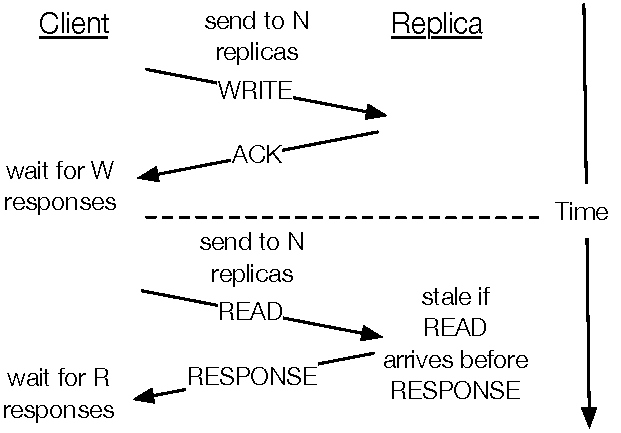
\includegraphics[width=.8\columnwidth]{figs/dynamostale.pdf}
\caption{The \textit{WARS}  model for message ordering in Dynamo describes the
  message flow between a coordinator and a single replica for a write
  followed by a read $t$ seconds after commit.  Note that, in an $N$
  replica system, this message flow is replicated $N$ times between
  the coordinator and $N$ replicas.  Note that the read and write may be handled by different coordinators.}
\label{fig:dynamo-diagram}
\end{figure}

For a write, the coordinator sends $N$ messages, one to each
replica. The message from coordinator to replica containing the
version to be written is delayed by a value chosen from distribution
\texttt{W}.  The coordinator waits for $W$ responses from the replicas
before we can consider the version committed, each of which are delayed by
a value chosen from the distribution \texttt{A}.

For a read, the coordinator sends $N$ messages, one to each replica.
The message from coordinator to replica containing the read request is
delayed by a value chosen from distribution \texttt{R}.  The
coordinator waits for $R$ responses from the replicas before returning
the most recent value it recieves.  Each read response is delayed by a
value chosen from the distribution \texttt{S}.

In the absence of additional anti-entropic processes, the coordinator
will return stale data if all $R$ of the $N$ responses received before
the read returns reached their respective replicas before the
respective message delayed by \texttt{W} does.  When $R$$+$$W$$>$$N$,
this is impossible.  However, under partial quorums (when
$R$$+$$W$$\leq$$N$), this is potentially highly unlikely.  If we
denote the commit time as $w_t$, to observe staleness, $r+w_t < w$ for
$r$ chosen from \texttt{R} and $w$ chosen from \texttt{W}.  Writes
have time to propagate additional replicas as replicas acknowledge the
write and as reads are sent out.  Similarly, messages are further
delayed in transit (\texttt{S}) back to the read coordinator.
Qualitatively, longer write tails and faster reads increase the chance
of staleness due to the possibility of reordering.

Depending on which coordinator a client contacts, some reads and
writes may be served locally.  In this case, subject to local query
processing delays, a read or write to $R$ or $W$ nodes is behaves like
a read or write to $R-1$ or $W-1$ nodes, respectively.  Modeling
non-local (e.g., proxied) coordinators is a conservative analysis.

As we discussed in Section~\ref{sec:practice}, read repair and Merkle
tree anti-entropic processes decrease the probability of staleness by
further propagating versions between members.  However, both of these
processes are rate dependent: read repair effects depend on the rate
of reads, and Merkle tree exchange effects depend on the rate of
exchange.  \textit{WARS}  is read rate independent but is affected by the
write rate.  If multiple writes overlap, that is, have overlapping
periods where they are in-flight but are not committed, the
probability of inconsistency decreases.  Intuitively, this is because
overlapping writes only leads to an increased chance that a client
reads as-yet-uncommitted data.  Accordingly, because it does not
capture read repair or Merkle tree exchange, \textit{WARS}  represents a lower
bound for Dynamo-style operation for the sake of simplicity of
analysis.

K-STALENESS AND WRITE INDEPENDENCE

\textit{WARS}  considers the effect of message sending, delays, and reception,
but this represents a daunting analytical formulation.  The commit
time represents an order statistic dependent on both \texttt{W} and
\texttt{A}.  By itself, this is not problematic, but message
reordering is dependent on the commit time.  The probability that the
$i$th returned read message observes reordering is a both an order
statistic dependent on $W$ and $A$, and, between $i$, the
probabilities are dependent.  The expected read and write latencies can
be computed using simple order statistics if one makes independence
assumptions about the distributions in \textit{WARS} .  However, a concise,
closed form for the probability of inconsistency eludes.  Dynamo is
simple to reason about and program, but difficult to analyze in closed
form.  As we discuss in Section~\ref{sec:sim}, we explore \textit{WARS}  using
Monte Carlo analysis, which suffices for our purposes in practice and,
from a practical perspective, is relatively easier to implement.


\subsection{Asynchronous Staleness Detection}

Even if a system provides an extremely high probability of
consistency, it is may be useful if applications can be notified when
data returned is inconsistent, or staler than promised.  Thankfully,
the Dynamo model is naturally equipped for staleness detection.

Knowing whether a response is stale at read time requires strong
consistency.  For the purposes of an informal proof, assume staleness
detection did not require strong consistency.  By enumerating all
possible values in the domain and checking them against the staleness
detector, we could determine the consistent value.  Conversely, if we
do not have strong consistency, then we cannot determine the last
committed version. However, we \textit{can} determine staleness
asynchronously.  Asynchronous staleness detection allows speculative
execution~\cite{nsdispeculation} and if a program contains appropriate
compensation logic.

We first consider a staleness detector that provides false positives.
Recall that, in a Dynamo-style system, we wait for $R$ of $N$ replies
before returning a value.  The remaining $N-R$ replicas will still
reply to the read coordinator.  Instead of dropping these messages,
the coordinator can compare them to the version it returned.  If there
is a mismatch, then either the coordinator returned stale data, there
are in-flight writes in the system, or additional versions committed
after the read.  The latter two cases lead to false positives.  We
define staleness according to the last committed write when the read
began, so versions written after the last committed version do not
technically constitute stale reads.  Notifying clients of newer
versions of a data item is not necessarily bad but may be unnecessary
and violates our staleness semantics.  Note that this detector does
not require modifications to the Dynamo protocol, yet we believe this
is the first record of this property.

To eliminate false positives, we need to determine the total,
system-wide commit ordering of writes. Recall that replicas are
unaware of the commit time for each version; commits occur after $W$
replicas respond and the version stamps that replicas store are not
updated after commit.  To establish a total ordering, a single
designated write coordinator can serialize writes.  To guard against
failures (and subsequent loss of the ordering), the ordering log
should be reliably replicated using a reliable consensus algorithm
such as Paxos.  However, if the single write coordinator is a
bottleneck, we could use multiple write coordinators.  With the
presence of globally synchronized local clocks, coordinators could
gossip the mapping from versions to commit times or even write their
own commit times back to the replicas in another round-trip of
messages.  Without globally synchronized local clocks, the
coordinators could obtain a logical timestamp from a centralized
replica prior to committing (doing so after committing leads to
races).  Eliminating false positives requires modifications to the
Dynamo protocol but is definitely tractable.

While this discussion has been couched in the terms of strong
consistency, it is easily extended to PBS $k$-staleness and PBS
$\langle k, t \rangle$-staleness.

\section{Evaluating Dynamo $t$-visibility}
\label{sec:dynamoeval}

As discussed in Section~\ref{sec:tvis}, PBS $t$-visibility depends on
the propagation of reads and writes throughout a system.  We
introduced the \textit{WARS}  model as a means of reasoning about
inconsistency in Dynamo-style quorum systems, but quantitative metrics
such as staleness observed in practice depend on each of \textit{WARS} 's
latency distributions.  In this section, we perform an analysis of
Dynamo-style $t$-visibility under several different assumptions.  We
use a mix of real-world experiments on EC2 and Monte Carlo analyses
under internet-scale company production distributions to better
understand how frequently ``eventually consistent'' means
``consistent'' and, more importantly, why.

Recall that PBS $k$-staleness is easily captured in closed form for
static quorums.  In practice, with static quorums and no anti-entropy,
we observe that their equations hold true.  However, in a system
employing anti-entropy, we cannot disentangle time and versions.  In
this section, we focus mainly on $t$-visibility but briefly describe
some $\langle k, t \rangle$-staleness results.

In this section, we focus on worst-case bounds for staleness.  While
we could improve the staleness results by considering additional
anti-entropic processes, we make the bare minimum of assumptions as
dictated by the \textit{WARS}  model.  Opting for conservative analyses
decreases the number of varibles in our experiments (each of which is
supported by empirical observations from practicioners) and increases
the applicability of these results.

\subsection{Monte Carlo Simulator}

We implemented \textit{WARS}  in a simple event-driven simulation environment.
Calculating $t$-visibility for a given value of $t$ is rather
straightforward: draw $N$ samples from \texttt{W}, \texttt{A},
\texttt{R}, and \texttt{S} at time $t$ (denote index $i$ as $[i]$), compute $w_t = \texttt{W}[W]+\texttt{A}[W]$, and check whether the
first $R$ samples of \texttt{R}, ordered by
$\texttt{R}[i]+\texttt{S}[i]$ obey $w_t+\texttt{R}[i] \leq
\texttt{W}[i]$.  This requires only a few lines of code.  Implementing
$\langle k, t \rangle$-staleness requires remembering write ordering
and history but is not difficult.

\subsection{Model Validation}

To validate \textit{WARS}  (and our subsequent analyses), we instrumented a
commercially available, open source Dynamo-style key-value store to
measure the staleness observed under partial quorum operation.
Unsurprisingly, our observations matched \textit{WARS}.

We modified Cassandra, a data store originally designed at Facebook,
which provides Dynamo-style partial quorum semantics, offering
per-request quorum sizes and a BigTable-like data
model~\cite{cassandra, cassandra-sigmod}.  Our changes to Cassandra were minimal:
we added support for partial quorums of size greater than
three---requiring changes to the wire protocol and request handling
code---and instrumented parts of the database to provide timing
information about reads and writes.  By analyzing Cassandra logs, we
were able to reconstruct the latency distributions of write requests,
write acknowledgements, read requests, and read responses.  We
disabled read repair because \textit{WARS} is read-rate independent.

We deployed Cassandra on Amazon EC2 and compared the observed
staleness to our predicted staleness for a number of configurations.
To provide a single point of order for the series of reads and writes
in the system, we deployed $N+1$ Cassandra nodes for each experiment
involving $N$ nodes.  After configuring the Cassandra schema, we
determined the node that did not store the data and sent all requests
through it, effectively creating a remote proxy.  \textit{WARS}  is more
general than the specific proxy configuration, however using a
centralized proxy allows us to avoid most issues with clock skew
between replicas and rely less heavily on globally synchronized
clocks.

We used \texttt{m1.small} instances throughout our experiments within
the \texttt{us-east-1} availability zone.  We ran a single reader and
a single writer to a monotonically increasing key in Cassandra and
compare the read and write timestamps to predict the staleness.  This
is not necessarily representative, so to model network and remote
processing delays, we injected various delays into both the request
and response sending modules in Cassandra (we discuss a range of
distributions in Section~\ref{sec:latencies}).  One major challenge in
performing our experiments was clock skew across replicas; we relied
on both \texttt{ntp} and userland skew measurements to bound these
drifts.  This is a recently studied problem, particularly under VM
migration and in the Xen hypervisor~\cite{time-virt}. In future
experiments, simulation avoided these complexities.

Across multiple latency profiles, we were able to predict staleness
with extremely high accuracy. Under default settings, we did not
observe any staleness due to the limited operation latency; message
reordering was not a problem.  Using the operation delays recorded in
Cassandra across 5000 writes, we reconstructed the latency
distributions and repeated each experiment in simulation.  On average,
our Monte Carlo simulations predicted $<k,t>$ staleness within XX\% of
the observed staleness.  As shown in Figure \ref{fig:fits}, our
simulation has no greater than YY\% inaccuracy for any given $<k,t>$
staleness prediction.  We attribute this inaccuracy to sample size.


\subsection{Latency Models}
\label{sec:latencies}

\textit{WARS} depends only on latency distributions, and, rather than
conjecture as to what represents ``reasonable'' scenarios, we analyzed
production distributions from two internet-scale companies, LinkedIn
and Yammer.

LinkedIn~\cite{linkedin} is an online professional social network
claiming over 135 million members as of November
2011~\cite{linkedinmembers}. To handle highly available, low latency
data storage, engineers at LinkedIn built Voldemort, a Dynamo-style
quorum replicated key value store~\cite{voldemort, voldemortpub}.
Alex Feinberg, a lead engineer on Voldemort, graciously provided us
with latency distributions for a single node replaying peak load
traffic for the ``Who Viewed My Profile?'' data set on LinkedIn,
representing 60\% read and 40\% read-modify-write traffic
(Table~\ref{table:linkedin})~\cite{feinbergpc}.  Feinberg reports that
``with spinning disks, we're largely IO bound and latency is largely
determined by the kind of disks we're using, data to memory ratio and
request distribution.  With [solid state drives (SSDs)], we're CPU
and/or network bound (depending on value size).''  As an interesting
aside, Feinberg also notes that ``maximum latency is generally
determined by GC activity (rare, but happens occasionally) and is
within hundreds of milliseconds.''

\begin{table}[h!]
\begin{center}
\begin{tabular}{|c|c|}
\hline
\%ile & Latency (ms) \\
\hline
\multicolumn{2}{|c|}{ 15,000 RPM SAS Disk}\\
\hline
Average & 4.85\\
95 & 15\\
99 & 25\\
\hline
\multicolumn{2}{|c|}{ Commodity SSD }\\
\hline
Average & 0.58 \\
95 & 1\\
99 & 2\\
\hline
\end{tabular}
\caption{LinkedIn Voldemort single-node production latencies.}
\label{table:linkedin}
\end{center}
\end{table}

Yammer is an online social network designed to provide enterprises
with private social networking capabilities.  As of December 2011,
Yammer claimed over 100,000 companies as customers~\cite{yammer}.
Yammer uses Basho's Riak, another open source Dynamo-style quorum
replicated database for client data~\cite{riak}.  Coda Hale,
infrastructure architect, and Ryan Kennedy, also of Yammer, presented
on their use of Riak including surprisingly in-depth performance
numbers in March 2011~\cite{riakyammer}.  Yammer provided us with more
detailed performance numbers for their application
(Table~\ref{table:yammer})~\cite{codapc}.  Coda noted that ``reads and
writes have radically different expected latencies, especially for
Riak. Writes don't return until the fsync returns, so while reads are
often $<$ 1ms, writes rarely are.''  As we will see, this has
important consequences for \textit{WARS}.  Although we do not model
this explicitly, Coda also notes that ``value size is also
interesting. We saw a big performance improvement by adding LZF
compression to values.''

\begin{table}[h!]
\begin{center}
\begin{tabular}{|c|c|c|}
\hline
\%ile & Read Latency (ms) & Write Latency (ms)\\
\hline
Min & 1.55 & 1.68\\
50 & 3.75 & 5.73 \\
75 & 4.17 & 6.50\\
95 & 5.2 & 8.48\\
98 & 6.045 & 10.36 \\
99 & 6.59 & 131.73\\
99.9 & 32.89 & 435.83\\
Max & 2979.85 &  4465.28 \\
\hline
Mean & 9.23 & 8.62 \\
Std. Dev. & 83.93 & 26.10\\
\hline
Mean Rate & 718.18 gets/s & 45.65 puts/s\\
\hline
\end{tabular}
\caption{Yammer Riak $N$$=$$3$, $R$$=$$2$, $W$$=$$2$ production latencies.}
\label{table:yammer}
\end{center}
\end{table}

These production data are invaluable, yet they are underspecified for
\textit{WARS}.  First, they are summary statistics, so we need to
calculate the underlying distribution.  More importantly, the
operation latencies represent round-trip times, while \textit{WARS}
requires the constituent one-way latencies for reads and writes.
Accordingly, to derive \texttt{W},\texttt{A},\texttt{R},\texttt{S} for
each configuration, we made a series of assumptions.  These
assumptions are imperfect, and do not perfectly mirror the real world.
As we demonstrated in our Cassandra experiments, these latency
distributions are easily collected.  However, because they are not
currently collected in practice, we must do our best to fill in the
gaps.  When possible, we are conservative in our fits by understating
write latencies and overstating other latencies.  We believe that
these assumptions are justified given the advantage of production data
over synthetic distributions and, when relevant, we supplement our
experimental setup with synthetic distributions.  Without additional
data on the latency required to read multiple replicas, we assume that
each latency distribution is independently, identically distributed.

LinkedIn provided two latency distributions, which we denote
\texttt{LNKD-SSD} and \texttt{LNKD-DISK} for the SSD and spinning
disks, respectively.  As previously discussed, when running on SSDs,
Voldemort is largely network and CPU bound.  Accordingly, we assumed
that read and write operations took equivalent amounts of time and, to
split the remaining time, we focused on the network-bound case and
assumed that one-way trips were symmetric
(\texttt{W}=\texttt{A}=\texttt{R}=\texttt{S}).  This allowed us to
derive \texttt{LNKD-SSD}.  For \texttt{LNKD-DISK}, Feinberg mentioned
that Voldemort performs at least one read before every write (average
of 1 seek, between 1-3 seeks), and writes to the BerkeleyDB Java
Edition backend are flushed every 30 seconds or 20
megabytes---whichever comes first.  Accordingly, we kept the same
\texttt{A}=\texttt{R}=\texttt{S} as in \texttt{LNKD-SSD} but
calculated \texttt{W} separately.  We discussed our methodology with
Feinberg, who approved of these assumptions.  Both of the
distributions were exponentially distributed:\vspace{-2mm}

\begin{equation*}
 \begin{array}{rll}
\texttt{LNKD-SSD} \rightarrow & \texttt{W} = \texttt{A}= \texttt{R} = \texttt{S}: & \lambda = 3.28\\
\texttt{LNKD-DISK} \rightarrow & \texttt{W}: & \lambda = .1861\\
&  \texttt{A} = \texttt{R} = \texttt{S}: & \lambda = 3.28$$\\
\end{array}
\end{equation*}

Yammer provided distributions for a single configuration but separated
read from write latencies, which we denote \texttt{YMMR}.  Using our
IID assumptions, we fit single-node latency distributions to the
provided distributions, again assuming symmetric \texttt{A},
\texttt{R}, and \texttt{S}.  The data fit a Pareto distribution,
although we opted to fit the body latencies ($p<.99)$ over the tail
latencies.  A mixed Gaussian distribution would help solve this
problem.\vspace{-2mm}

\begin{equation*}
 \begin{array}{rll}
   \texttt{YMMR} \rightarrow  & \texttt{W}: & x_m = 2.7, \alpha=2.34\\
     & \texttt{A}= \texttt{R} = \texttt{S}: & x_m=1.385, \alpha=2.866\\
    \end{array}
\end{equation*}


\begin{figure*}
\centering
\subfigure{
\includegraphics[width=\columnwidth]{figs/latlegend.pdf}}\\[-1mm]
\subfigure{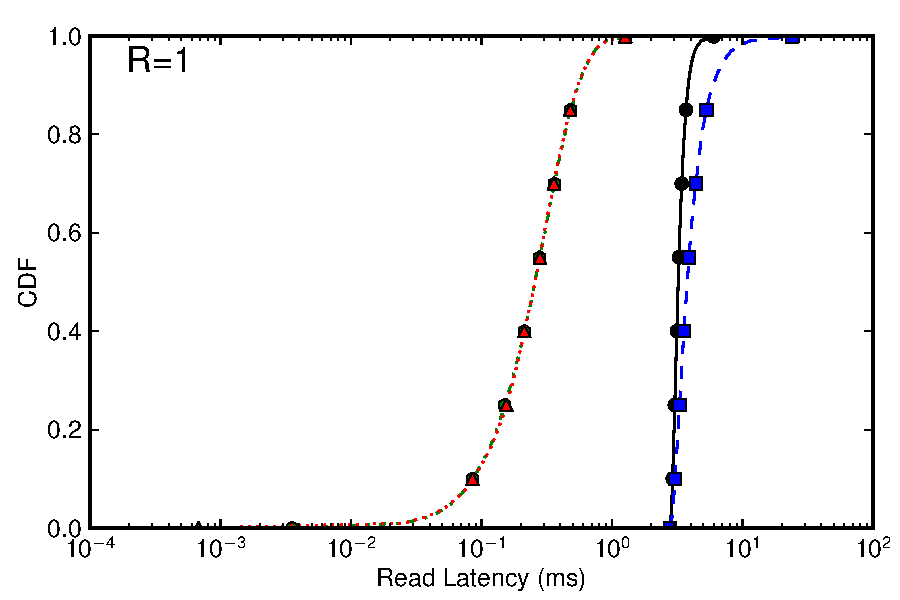
\includegraphics[width=.6\columnwidth]{figs/readlats-1.pdf}}
\subfigure{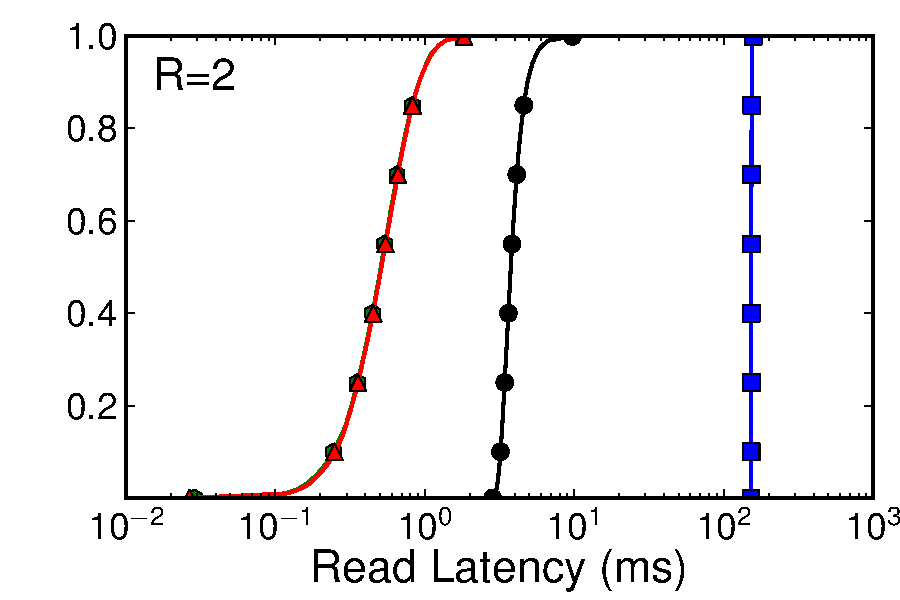
\includegraphics[width=.6\columnwidth]{figs/readlats-2.pdf}}
\subfigure{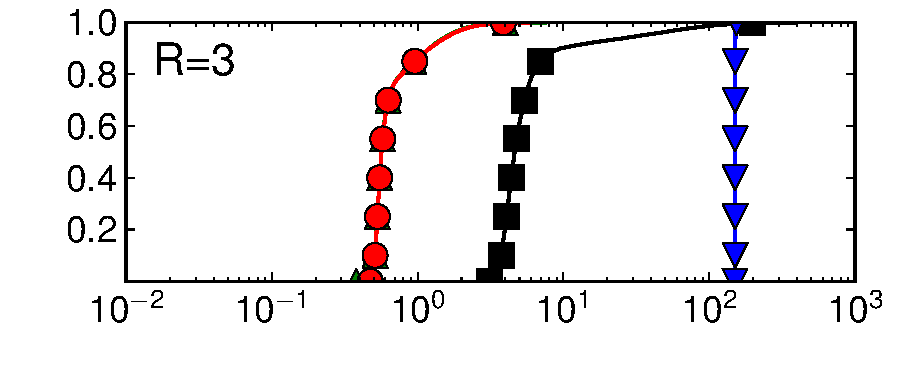
\includegraphics[width=.6\columnwidth]{figs/readlats-3.pdf}}
\subfigure{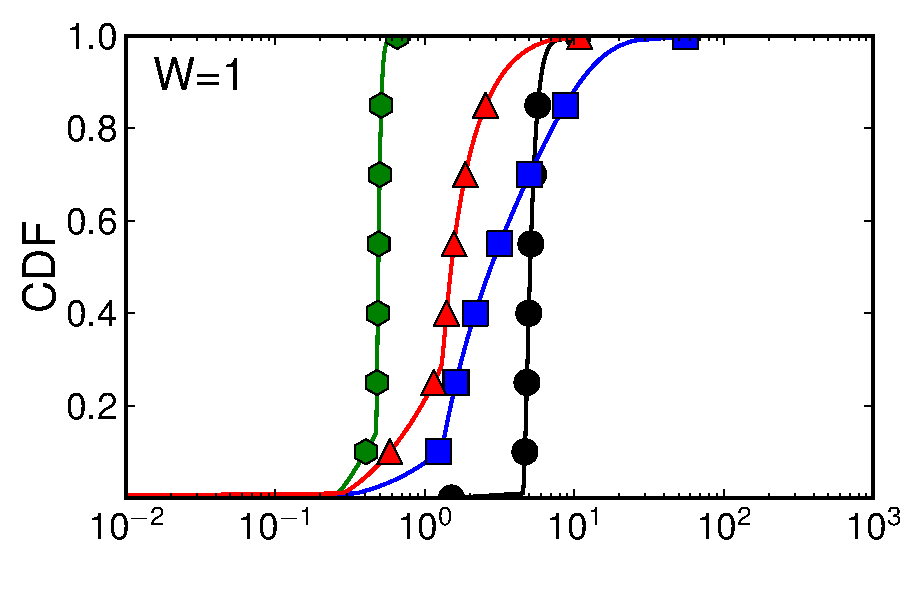
\includegraphics[width=.6\columnwidth]{figs/writelats-1.pdf}}
\subfigure{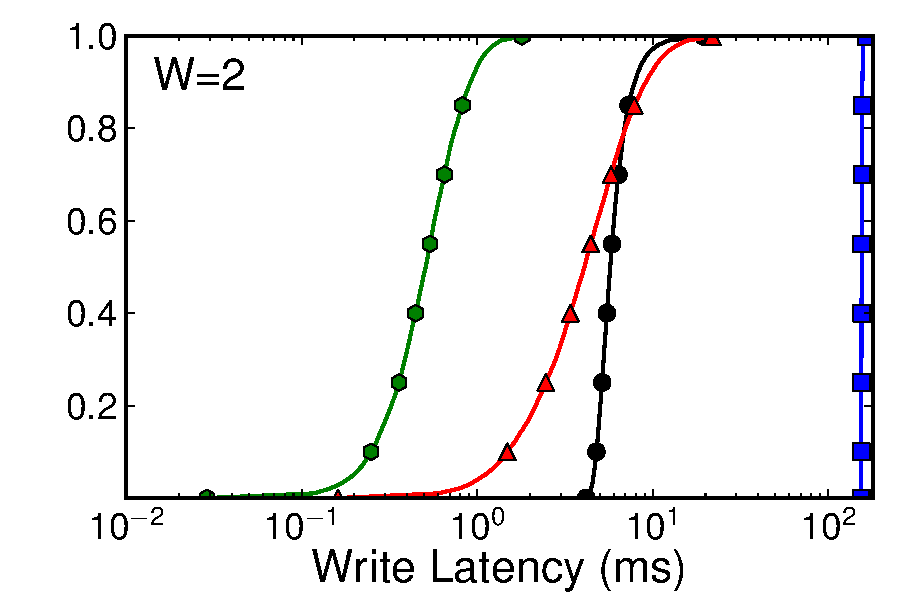
\includegraphics[width=.6\columnwidth]{figs/writelats-2.pdf}}
\subfigure{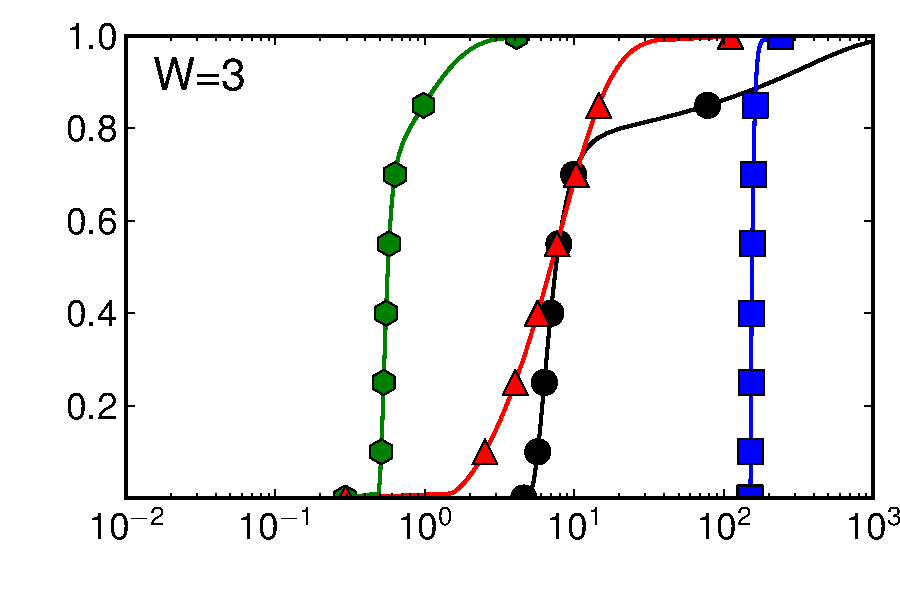
\includegraphics[width=.6\columnwidth]{figs/writelats-3.pdf}}
\caption{Read and write operation latency for \textit{WARS} latencies fitted
  to production datasets for $N$$=$$3$.}
\label{fig:latencies}
\end{figure*}

Finally, we simulated a normal-case WAN replication scenario,
\texttt{WAN}.  Reads and writes are routed to random data centers,
and, accordingly, one replica operation commits quickly while the
others are routed remotely.  We delay remote operations by 75ms and
apply \texttt{YMMR} delays once the operation reaches its target data center.

We plot each fitted distribution in Figure~\ref{fig:latencies}.  Note
that for $R$, $W$ of one, \texttt{YMMR} is not equivalent to
\texttt{WAN}.  This is because, in \texttt{YMMR}, we only have to wait
for the first of $N$ local reads (writes) to return, whereas there is
only one local read (write) in \texttt{WAN}, and all other read
(write) requests will be delayed at least 150ms.

\subsection{Observed $t$-visibility}

We measured the $t$-visibility for each distribution
(Figure~\ref{fig:tvis}).  By issuing simulating a series of reads
after each of 1000 non-overlapping writes staggered by time (as
plotted 10 reads each), we calculated the probability of consistency,
or $t$-visibility across time.

The high probability of consistency was largely dependent on the write
tail size.  Immediately after writing, \texttt{YMMR} had a $88\%$
chance of consistency, \texttt{LNKD-SSD} had a $75\%$ chance, and
\texttt{LNKD-DISK} had a $39\%$ chance.  However, one millisecond
after writing, \texttt{YMMR} had a $91.5\%$ chance of consistency,
\texttt{LNKD-SSD} had a $99\%$ chance, and \texttt{LNKD-DISK} had a
$48\%$ chance.  \texttt{YMMR}'s tall body but long tail limited its
probability increase, and only reached $99.9\%$ consistency 44ms after
writing.  \texttt{LNKD-SSD}'s reads raced its writes immediately after
commit, but, one millisecond after the write, the chance of a read
round-trip time plus one millisecond beating its write was almost
eliminated.  \texttt{LNKD-DISK} had the longest body of these three
distributions and only reached $99.9\%$ confidence after 39ms (having
a shorter tail than \texttt{YMMR}).  As expected, \texttt{WAN}
observed poor chances of consistency until after the 75 milliseconds
passed; unless a reader read from the same datacenter in which the
last write committed, it had to wait for the long propagation to
observe the most recent value.

\begin{figure*}
\centering
\subfigure{
\includegraphics[width=\columnwidth]{figs/latlegend.pdf}}\\[-1mm]
\subfigure{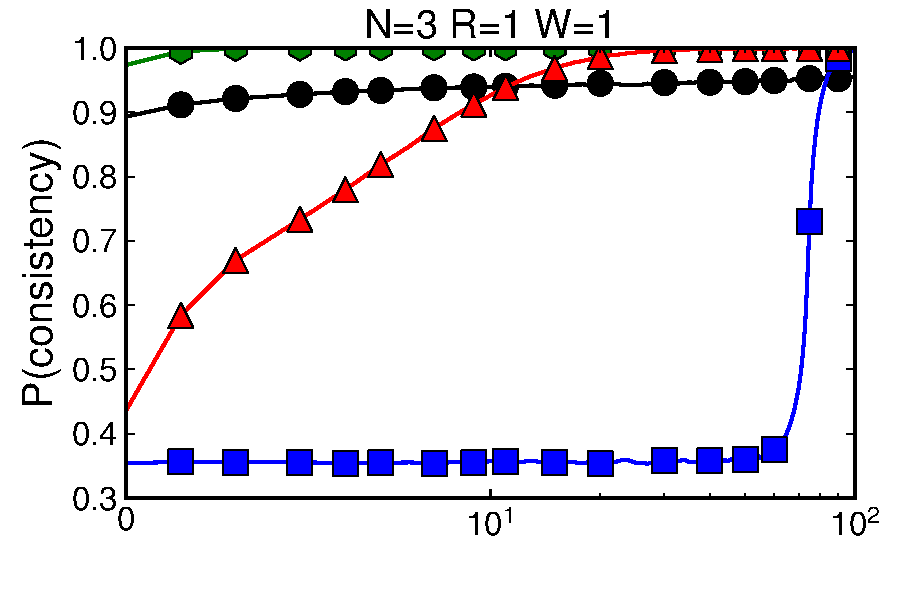
\includegraphics[width=.65\columnwidth]{figs/tstales-3N1R1W.pdf}}
\subfigure{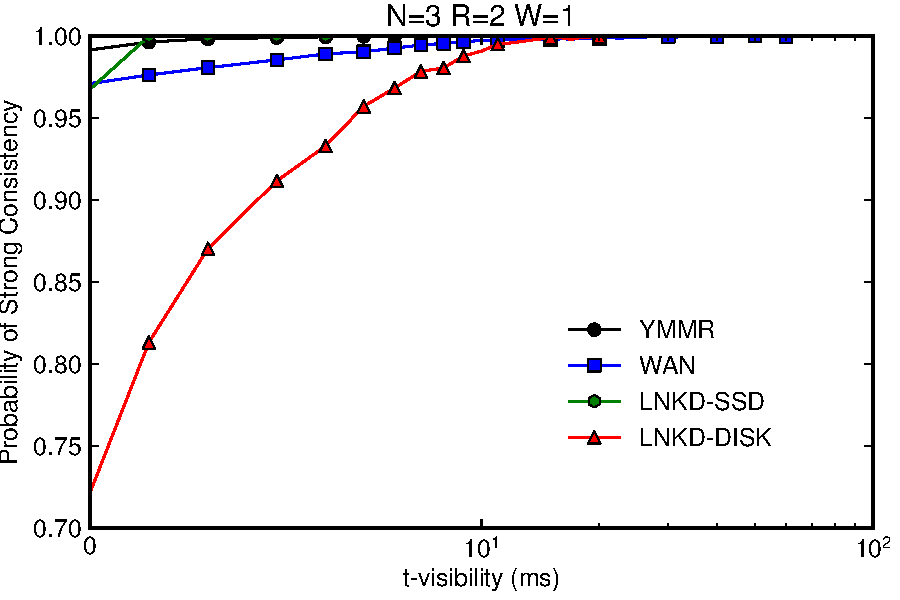
\includegraphics[width=.65\columnwidth]{figs/tstales-3N2R1W.pdf}}
\subfigure{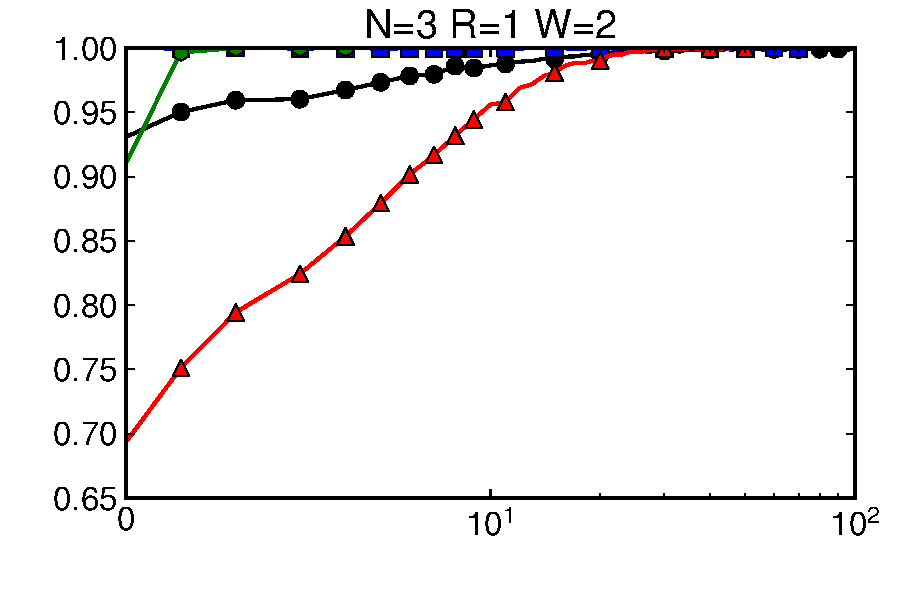
\includegraphics[width=.65\columnwidth]{figs/tstales-3N1R2W.pdf}}
\caption{$t$-visibility for production operation latencies.}
\label{fig:tvis}
\end{figure*}

As \textit{WARS} predicted, the ratio of \texttt{W} to
\texttt{A}=\texttt{R}=\texttt{S} largely influenced the probability of
consistency.  As shown in Figure~\ref{fig:varydelay}, we swept a range
of exponential distributions, fixing \texttt{A}=\texttt{R}=\texttt{S}
and varying \texttt{W}.  When the mean of \texttt{W} ($.25$ms) is
one-fourth the mean of \texttt{A}=\textit{R}\textit{S}, we observe a
$94\%$ chance of consistency immediately after the write and $99.9\%$
chance after 1ms.  However, when the mean of \texttt{W} ($10$ms) is
ten times the mean of \texttt{A}=\texttt{R}=\texttt{S}, we observe a
$41\%$ chance of consistency immediately after write and a $99.9\%$
chance of consistency after $65$ms.

\begin{figure}
\centering
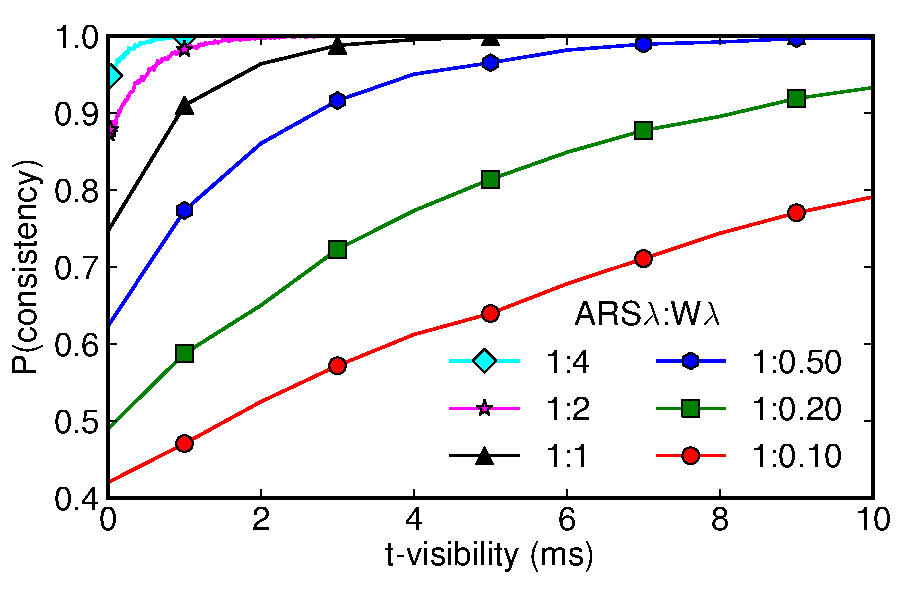
\includegraphics[width=.85\columnwidth]{figs/rwratio.pdf}
\caption{$t$-staleness for $N$$=$$3$, $R$$=$$W$$=$$1$ varying \texttt{W} and \texttt{A}=\texttt{R}=\texttt{S} exponentially distributed delays.  Mean latency is $1/\lambda$.}
\label{fig:varydelay}
\end{figure}

These data strongly suggest that operators should strive to lower
(relative) \texttt{W} latencies.  While databases could artificially
delay read latencies, this is problematic for read-heavy workloads and
potentially introduces queuing effects for reads and writes.

For $N$ greater than three, $R$$=$$W$$=$$1$ leads to increased
staleness (Figure~\ref{fig:varyn}).  



\begin{figure*}
\centering
\subfigure{\includegraphics[width=.65\columnwidth]{figs/sweepn-LNKD-DISK.pdf}}
\subfigure{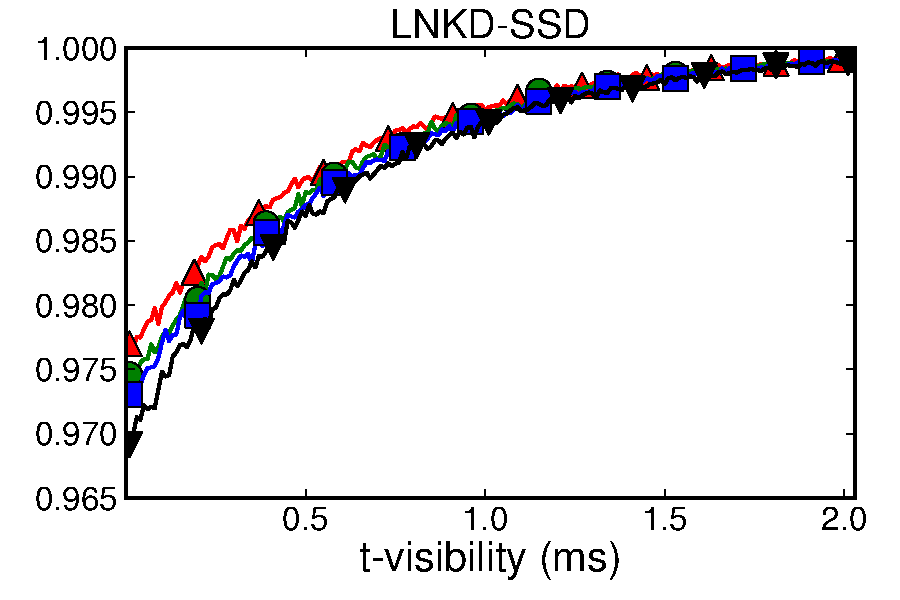
\includegraphics[width=.65\columnwidth]{figs/sweepn-LNKD-SSD.pdf}}
\subfigure{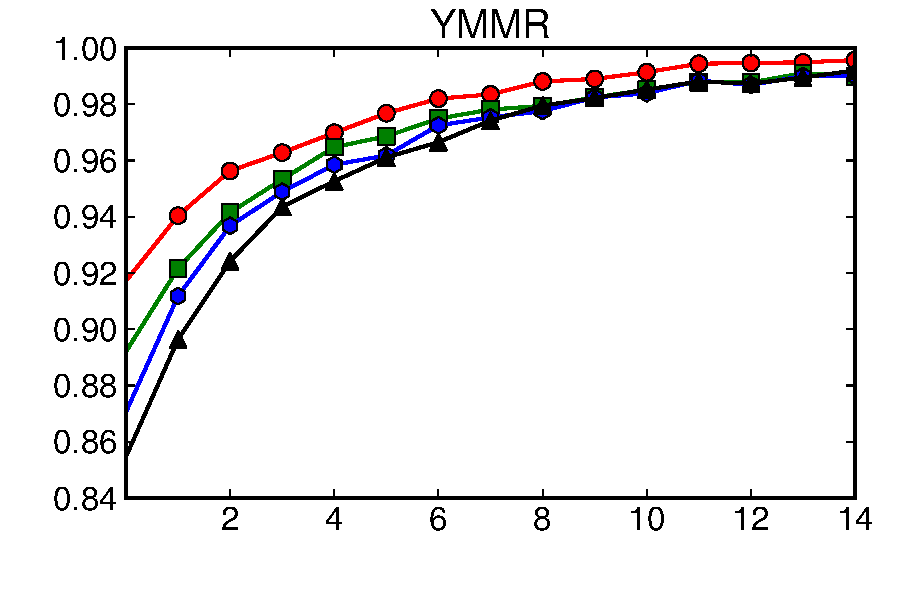
\includegraphics[width=.65\columnwidth]{figs/sweepn-YMMR.pdf}}
\caption{$t$-visibility for production operating latencies for variable $N$ and $R$$=$$W$$=$$1$.}
\label{fig:varyn}
\end{figure*}


Table~\ref{table:lat-stale} shows latencies and $t$-visibility for a $99.9\%$ probability of strong consistency.

\begin{table*}
\begin{center}
\begin{tabular}{c|c|c|c|c|c|c|c|c|c|c|c|c|}
\cline{2-13}
& \multicolumn{2}{|c|}{$R$$=$$1$, $W$$=$$1$} & \multicolumn{2}{|c|}{$R$$=$$1$, $W$$=$$2$} & \multicolumn{2}{|c|}{$R$$=$$1$, $W$$=$$3$} & \multicolumn{2}{|c|}{$R$$=$$2$, $W$$=$$1$} & \multicolumn{2}{|c|}{$R$$=$$2$, $W$$=$$2$} & \multicolumn{2}{|c|}{$R$$=$$3$, $W$$=$$1$}  \\
&\multicolumn{1}{|c}{latency} & \multicolumn{1}{c|}{$t$} &  \multicolumn{1}{|c}{latency} & \multicolumn{1}{c|}{$t$} &  \multicolumn{1}{|c}{latency} & \multicolumn{1}{c|}{$t$} &  \multicolumn{1}{|c}{latency} & \multicolumn{1}{c|}{$t$} &  \multicolumn{1}{|c}{latency} & \multicolumn{1}{c|}{$t$} &  \multicolumn{1}{|c}{latency} & \multicolumn{1}{c|}{$t$}   \\ \hline
\multicolumn{1}{|c|}{\texttt{YMMR}} & 
16.19 & 44.0 & 23.43 & 33.0 & 83.41 & 0 & 17.57 & 3.0 & 39.39 & 0 & 55.56 & 0  \\
\multicolumn{1}{|c|}{\texttt{WAN}} & 
120.04 & 103.0 & 183.61 & 0 & 288.49 & 0 & 202.75 & 23.0 & 326.0 & 0 & 217.57 & 0 \\
\multicolumn{1}{|c|}{\texttt{LNKD-SSD}} & 
2.42 & 2.0 & 2.79 & 2.0 & 5.01 & 0 & 2.67 & 1.0 & 4.02 & 0 & 3.97 & 0  \\
\multicolumn{1}{|c|}{\texttt{LNKD-DISK}} & 
17.75 & 35.0 & 23.4 & 30.0 & 43.11 & 0 & 11.6 & 14.0 & 22.61 & 0 & 17.79 & 0  \\
\hline
\end{tabular}
\caption{$t$-visibility for $p_{staler} = .001$ ($99.9\%$ probability of consistency) and $99.9\%$ read plus write latency (equal weighting) across $R$ and $W$, $N$$=$$3$.}
\label{table:lat-stale}
\end{center}
\end{table*}


\section{Discussion}
\label{sec:discussion}

There are several aspects of distributed data systems that we have not yet
addressed.  Here, we briefly discuss improvements to our models.

\subsection{Is Eventually Consistent Good Enough?}

One Cassandra committer noted that although he had a patch for session guarantees, no Cassandra users had requested the functionality or claimed to require it.

\subsection{Additional Functionality}

READ-MODIFY-WRITE

\textbf{Staleness detection.} Each of the $p_{staler}$ bounds
describes a probability that a particular key is no staler than
specified.  In the context of probabilistic consistency SLAs, it would
be useful to determine whether a key is staler than promised by a
given SLA.  Determining this fact on-line is tantamount to achieving
strong consistency, however there are at least two strategies for
mitigating this difficulty. First, additional gossiping such as
regular negative acknowledgements can notify nodes of potential
version staleness.  This strategy has been discussed in the
literature~\cite{tocite} for non-probabilistic quorum systems.
Second, the system can provide asychronous notifications of staleness
information.  Proxies can keep a growing log of versions which, with
appropriate timestamping, can be used to determine if previously
returned values were staler than promised.  This is fairly
straightforward but requires careful garbage collection to manage
proxy-side state as the number of client requests scales.
Additionally, the possibility of proxy failure requires that prior
operations be durably logged; however, provided the proxy eventually
comes online and updates its log, the asynchronous guarantee holds.
Both of these schemes are feasible yet add significant complexity to a
probabilistically consistent quorum system.

\textbf{Multi-key transactions.} We have considered single-key operations,
however the ability to perform distributed transactions is potentially
attractive.  For read-only transactions, if the key distribution is
random, each quorum is independent, so we can simply multiple the
staleness probabilities of each key.  Achieving atomicity of writes to
multiple keys requires more complicated coordination mechanisms such
as two-phase commit.  Again, transactions are feasible but require
considerable care in implementation, complicated what is otherwise a
simple replication scheme.

\textbf{Node failures.} Fail-stop node failures can be easily
incorporated into our latency models. The probability of a node
permanently failing $p_{f-perm}$ can be represented by setting the
probability of infinitely long read and write
operations. $L_{w}(\inf)=L_{r}(\inf)=p_{f-perm}$.  Intermittent node
failures of length $t_{fail}$ can be represented by setting
$L_{w}(t_{fail})$ to the probability of the node failing.  In this
way, operation latency captures all expected failure semantics.

\textbf{Read repair and active anti-entropy.} Modern Dynamo-style
systems use a technique known as \textit{read repair} to reconcile
divergent versions at query-time.  If two nodes return different
responses to a \textit{get} request, the responses are merged and
forwarded to the determined out-of-date node.  Dynamo performs
additional anti-entropy using Merkle trees, however the open source
databases we have examined only perform read repair (CITATION
needed--at least Cassandra does this). We do not model read repair or
additional anti-entropy processes here (although doing so requires
only minimal changes to our model), so we overestimate the chance of
staleness violation.

\textbf{Variable $w$.} We have assumed the use of a single $w$ across
all writes.  However, many KVSs such as Cassandra and Riak allow the
use of per-operation consistency\footnote{Voldemort specifies
  consistency requirements at the schema level. This is ostensibly an
  engineering decision that could be changed with minimal
  modifications to the wire protocol.}

\textbf{99th Percentile Latency.}


STRONGER THAN STALENESS?  Cite Ayer as pathological case ``this is reflected in xx work on k-staleness because of etc. etc. etc.''


\section{Related Work}
\label{sec:relatedwork}

Theory

Vadhat

\section{Conclusion}
\label{sec:conclusion}

\begin{comment}
\section*{Acknowledgements}

Alex Feinberg
Coda Hale

Andy Gross
Justin Sheehy

Doug Terry

Sam Madden
Christopher Re
Marcos Aguilera

Eric Brewer

Greg Durrett
Greg Valiant


Ali Ghodsi

Peter Alvaro
Bill Marczak
Neil Conway
Hariyadi Gunawi

Bryan Kate

Patrick Wendell
Kay Ousterhout

\end{comment}

\balance

\bibliographystyle{abbrv}
\bibliography{ernst}

\begin{comment}
\begin{appendix}
\section{Dynamo-style Staleness}

We present an analytical closed-form solution to $p_{staler}$ for
$t$-visible partial quorums unde Dynamo-style.  What is the
probability that a read result is not strongly consistent (that is,
does not return the most recent value when the read began)? In this
section, when we refer to the ``last committed version'', we are
referring to the last committed version before the read began. We
consider the pathological case where a read occurs immediately after a
write occurs.

We assume that each writes to a replica is independently delayed by a
randomly distributed variate $W$, each write acknowledgement from a
replica to a writer is independently delayed by a randomly distributed
variate $A$, each read request to a replica is independently delayed
by a randomly distributed variate $R$, and each read response from a
replica to a reader is delayed according to a randomly distributed
variate $S$.  We make no assumptions as to the distribution of $W,$
$A,$ $R,$ and $S$, except that their domain is strictly positive (no
negative delay) and that values drawn from each are independently,
identically distributed (IID).

The probability that a read quorum does not contain the last committed
version is equivalent to the probability that each of the first $R$
read responses are all stale.  Denote the probability that the $i$th
response is stale as $stale_i$:
\begin{equation*}
p_{staler} = \prod_{i=0}^{R} \Pr(stale_i)
\end{equation*}

Denote the return time of the $i$th read response as $S_i$.  The probability that the $i$th response is stale is given by:
\begin{equation*}
\Pr(stale_i) = \int_{0}^{\infty} \Pr(S_i = t) \cdot \Pr(stale_i \mid S_i = t) dt
\end{equation*}

We can use simple order statistics to calculate the return time of the $i$th read response:
\begin{multline*}
\Pr(S_i = t) = \frac{N!}{(i-1)!(N-i)!}\cdot[\Pr(R+S< t)]^{i-1}\\\cdot\Pr(R+S = t)\cdot[\Pr(R+S > t)]^{N-i}
\end{multline*}

 Recall that under Dynamo-style messaging, read response from a
 replica is stale if the read request arrived at the replica before
 the write command for the last committed version reached the replica.
 Denote the time required to commit the last version (alternatively, the time required for $W$ of $N$ replicas to acknowledge the last write) as $w_t$.
\begin{multline*}
\Pr(stale_i \mid S_i = t) = \int_{0}^{t} \Pr(R=\tau)\cdot\Pr(S=t-\tau)\\\cdot\Pr(R+w_t < W \mid R = \tau) d\tau
\end{multline*}
\begin{multline*}
  \Pr(R+w_t < W \mid R = \tau) = \int_{\tau}^{\infty} \Pr(W-w_t = x) dx
\end{multline*}
\begin{multline*}
  \Pr(W-w_t = z) = \int_{0}^{\infty} \Pr(W = y) \cdot \Pr(-w_t = z-y) dy
\end{multline*}
Finally, to calculate $w_t$, we calculate the probabilty that
$\mathcal{W}$ of $N$ acknowledgements come in at time $t$:
\begin{multline*}
\Pr(w_t = t) = \frac{N!}{(\mathcal{W}-1)!(N-\mathcal{W})!}\cdot[\Pr(W+A< t)]^{\mathcal{W}-1}\\\cdot\Pr(W+A = t)\cdot[\Pr(W+A > t)]^{N-\mathcal{W}}
\end{multline*}
Combining these equations, we have a closed-form solution for the
staleness dependent on $W,$ $A,$ $R,$ and $S$, as desired.  To consider
multiple version staleness, exponentiate $p_s$ by the number of
versions stale.

\end{appendix}
\end{comment}

\end{document}

